\documentclass[11pt]{article}
\usepackage[letterpaper,margin=1in]{geometry}
\usepackage[T1]{fontenc}
\usepackage[utf8]{inputenc}
\usepackage{lmodern}
\usepackage{amsmath,amssymb}
\usepackage{graphicx}
\usepackage{booktabs,tabularx}
\usepackage{enumitem}
\usepackage[font=small,labelfont=bf]{caption}
\usepackage{float}
\usepackage[colorlinks=true,linkcolor=blue!50!black,citecolor=blue!50!black,urlcolor=blue!50!black]{hyperref}
\usepackage{xcolor}
\usepackage[round]{natbib}

\graphicspath{{figures/}{../}}
\setlength{\parskip}{4pt}

\title{\textbf{Spiral Arms as Shocks:}\\ Gas Flow Through a Galactic Spiral Pattern}
\author{Aryana Haghjoo\\[2pt] \small Astrophysical Fluid Dynamics --- Final Project\\ \small University of California, Riverside}
\date{November 2026}

\begin{document}
\maketitle

\begin{abstract}
In density-wave theory, spiral arms are a pattern that rotates more slowly than the gas, so gas flows through the arms. We ask what the gas does when it meets an arm. Extending the finite-volume solver written for HW2 to a rotating, isothermal galactic disk, we find that the inflow is supersonic and the gas \emph{shocks}, forming narrow, dense arms, in agreement with the classic picture of \citet{roberts69}. The shocks are strongest where the inflow Mach number is highest and fade toward corotation. They sharpen for stronger spiral forcing and colder gas. The solver reproduces the exact isothermal jump condition $D=\mathcal{M}^2$ to within 2\%.
\end{abstract}

%=====================================================================
\section{How we started}
The starting idea was that ``spiral arms are waves in a fluid.'' That is partly true:
\begin{itemize}[nosep]
\item In \textbf{density-wave theory} \citep{linshu64}, the arms are a pattern that rotates at its own pattern speed $\Omega_p$, slower than the stars and gas. The wave itself lives mostly in the stellar disk.
\item The \textbf{gas} therefore overtakes the arms and flows \emph{through} them. It arrives faster than its sound speed, so it should shock \citep{roberts69}.
\end{itemize}
Simulating the stars self-consistently would require an $N$-body code. We instead study the part that fits a fluid-dynamics course: \textbf{the response of the gas} to a given spiral pattern. This lets us build directly on the Kelvin--Helmholtz code from HW2, and it ties together several course topics: finite-volume methods, the shock jump conditions (Ogilvie A.13) and oblique shocks (A.14).

%=====================================================================
\section{Model and assumptions}
We simulate a thin, face-on layer of gas in the frame rotating with the spiral pattern, so the arms are stationary. The equations are the isothermal Euler equations with gravity and rotating-frame forces:
\begin{align}
\frac{\partial\rho}{\partial t}+\nabla\cdot(\rho\mathbf{v}) &= 0,\\
\frac{\partial(\rho\mathbf{v})}{\partial t}+\nabla\cdot(\rho\mathbf{v}\mathbf{v})+c_s^2\nabla\rho &= -\rho\nabla(\Phi_0+\Phi_1)-2\rho\,\boldsymbol{\Omega}_p\times\mathbf{v}+\rho\,\Omega_p^2\,\mathbf{r},
\end{align}
with
\begin{equation}
\Phi_0=\tfrac12 v_0^2\ln(r^2+r_c^2),\qquad
\Phi_1=\epsilon\,v_0^2\cos\!\left[m\phi+m\cot i\,\ln r\right].
\end{equation}
$\Phi_0$ gives a flat rotation curve and $\Phi_1$ is a trailing, $m=2$ logarithmic spiral with pitch angle $i$. The perturbation amplitude is set by the forcing $F=m\epsilon\cot i$: the ratio of the spiral's radial force to the axisymmetric one. The main assumptions are summarized in Table~\ref{tab:assump}.

\begin{table}[H]
\centering\small
\begin{tabularx}{\textwidth}{@{}l l X@{}}
\toprule
Assumption & Choice & Reason \\
\midrule
Geometry & 2D, face-on disk & Arms are a disk phenomenon; 2D keeps runs fast \\
Gas & Isothermal, $c_s=0.05\,v_0\approx11$ km\,s$^{-1}$ & Interstellar gas cools quickly, so its temperature stays roughly fixed \\
Galaxy gravity & Fixed potential, flat rotation curve ($v_0=220$ km\,s$^{-1}$) & Matches real disk galaxies \\
Spiral & Imposed, $m=2$, $i=20^\circ$, $F=5\%$ & Typical of real spirals; we study the gas response, not arm formation \\
Pattern speed & $\Omega_p=0.9$: ILR at $r=0.33$, corotation at $r=1.11$ & Gas disk ($0.15<r<1$) lies where density-wave theory predicts arms \\
Left out & Self-gravity, magnetic fields, cooling, star formation & Keeps the problem focused on the shock \\
\bottomrule
\end{tabularx}
\caption{Model assumptions. Units: $R_0=10$ kpc, $v_0=220$ km\,s$^{-1}$, so one time unit is $44$ Myr.}
\label{tab:assump}
\end{table}

\begin{figure}[H]
\centering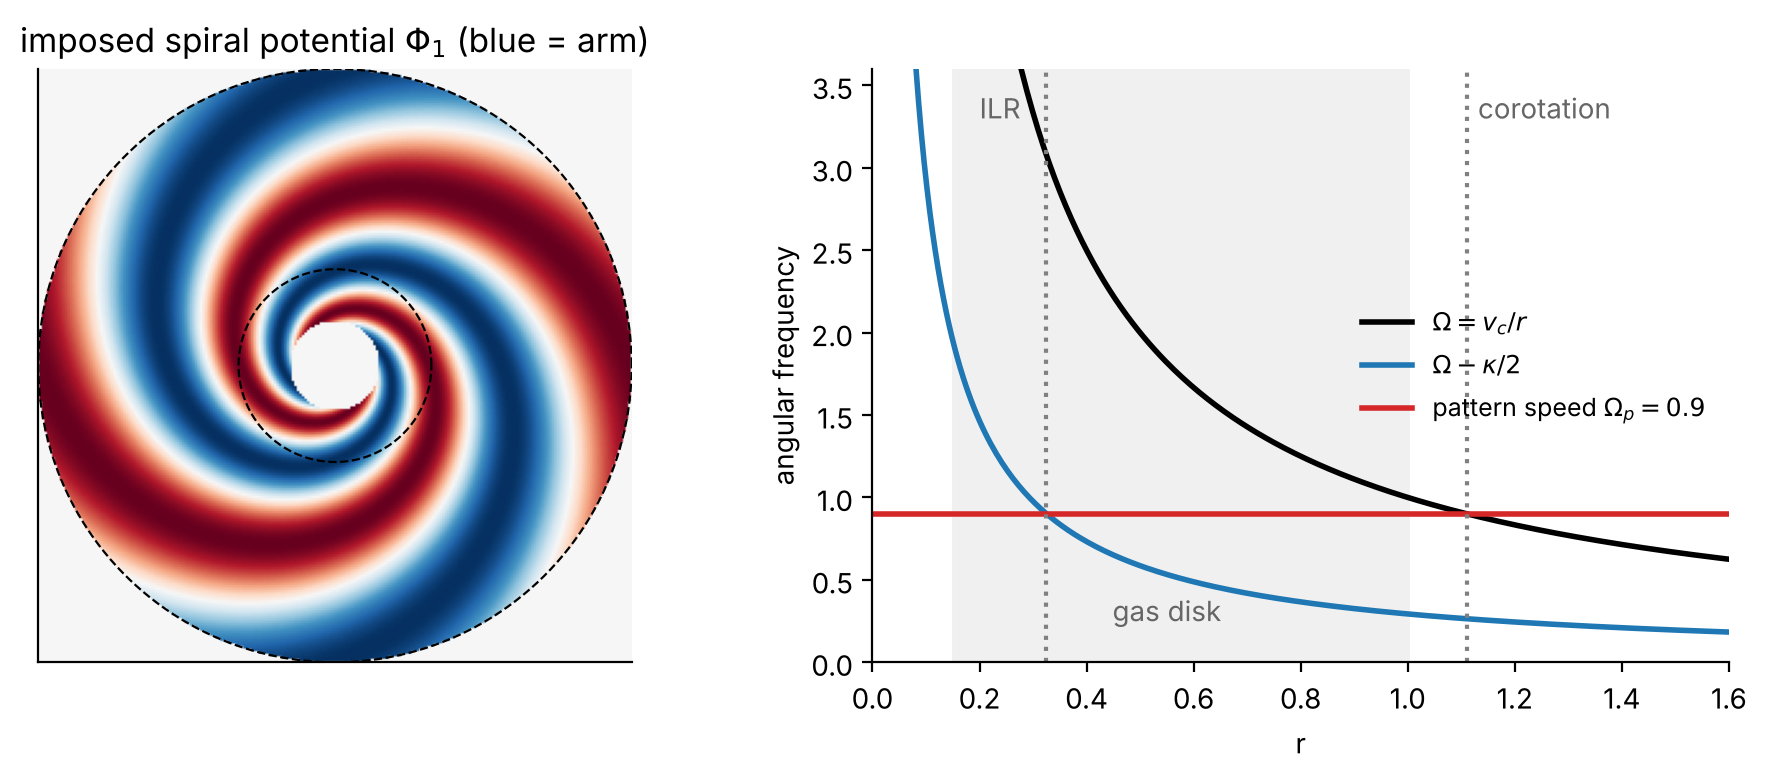
\includegraphics[width=0.95\textwidth]{fig_setup.png}
\caption{\textit{Left:} the imposed spiral potential $\Phi_1$ (blue = arm). \textit{Right:} angular frequency $\Omega$, $\Omega-\kappa/2$ and the pattern speed $\Omega_p$ versus radius, showing the inner Lindblad resonance (ILR) and corotation. The gas disk occupies the shaded region.}
\label{fig:setup}
\end{figure}

%=====================================================================
\section{Method}
\paragraph{The HW2 solver as the backbone.} The numerical core of the HW2 code (\texttt{kh\_sim.py}, a MUSCL--Hancock finite-volume scheme adapted from \citealt{mocz20}) is imported unchanged:
\begin{itemize}[nosep]
\item cell-centred gradients and the slope limiter;
\item the half-step predictor;
\item linear extrapolation to cell faces;
\item the conservative flux update with a CFL time step.
\end{itemize}
About 200 new lines (\texttt{spiral\_sim.py}) add the galaxy physics:
\begin{enumerate}[nosep]
\item an isothermal equation of state, $P=c_s^2\rho$, with the matching Rusanov flux;
\item time-centred gravity and rotating-frame source terms;
\item ``sponge'' zones at $r<0.2$ and $r>1$ that relax the gas toward its initial circular rotation, since the Cartesian grid is periodic but a galaxy is not.
\end{enumerate}
The spiral is switched on gradually over $t=3$ (130 Myr).

\paragraph{Runs.} The fiducial run uses $256^2$ cells on $[-1.1,1.1]^2$ and runs to $t=20$ (0.9 Gyr). That takes about 5{,}000 steps, or about 2 minutes on a laptop. We also varied:
\begin{itemize}[nosep]
\item the forcing, $F=0.5$--$10\%$;
\item the sound speed, $c_s=0.025$--$0.1$ ($\approx$ 6--22 km\,s$^{-1}$);
\item the resolution, $N=128$--$512$.
\end{itemize}

\paragraph{Verification.} We first tested the solver on two isothermal streams colliding at $\pm U$. Two shocks propagate outward and leave gas at rest between them. The jump conditions in the $\gamma\to1$ limit of A.13 give an exact solution:
\begin{equation}
D=\frac{\rho_2}{\rho_1}=\mathcal{M}_1^2,\qquad V_s=\tfrac12\left(\sqrt{U^2+4c_s^2}-U\right),\qquad \mathcal{M}_1=\frac{U+V_s}{c_s}.
\end{equation}
The simulated post-shock density matches this to within 2\% for $\mathcal{M}_1=1.6$--$6.2$, with shocks resolved in about 3 cells (Fig.~\ref{fig:verify}).

\begin{figure}[H]
\centering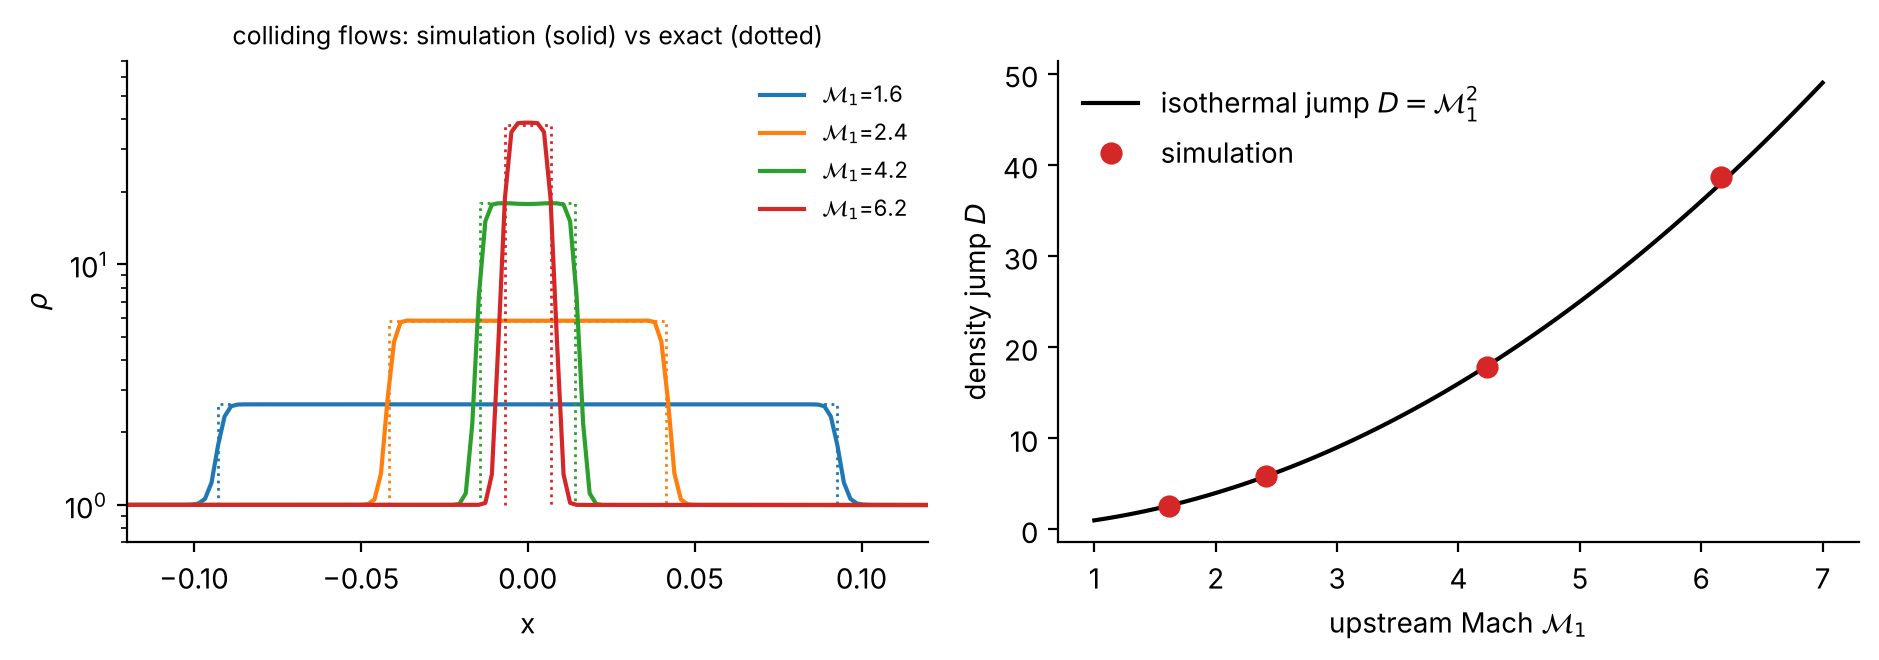
\includegraphics[width=0.95\textwidth]{fig_shocktest.png}
\caption{Verification. \textit{Left:} density profiles of the colliding-flow test (solid) against the exact solution (dotted). \textit{Right:} simulated density jump against the isothermal jump condition $D=\mathcal{M}_1^2$.}
\label{fig:verify}
\end{figure}

%=====================================================================
\section{Results}
\subsection{Arms form quickly and persist}
Narrow, dense spiral arms appear within about one ramp time (130 Myr), then settle into a quasi-steady pattern (Fig.~\ref{fig:snap}). The gas streams through the stationary pattern the whole time. In the inner disk the arm--interarm density contrast reaches $\approx 9$.

\begin{figure}[H]
\centering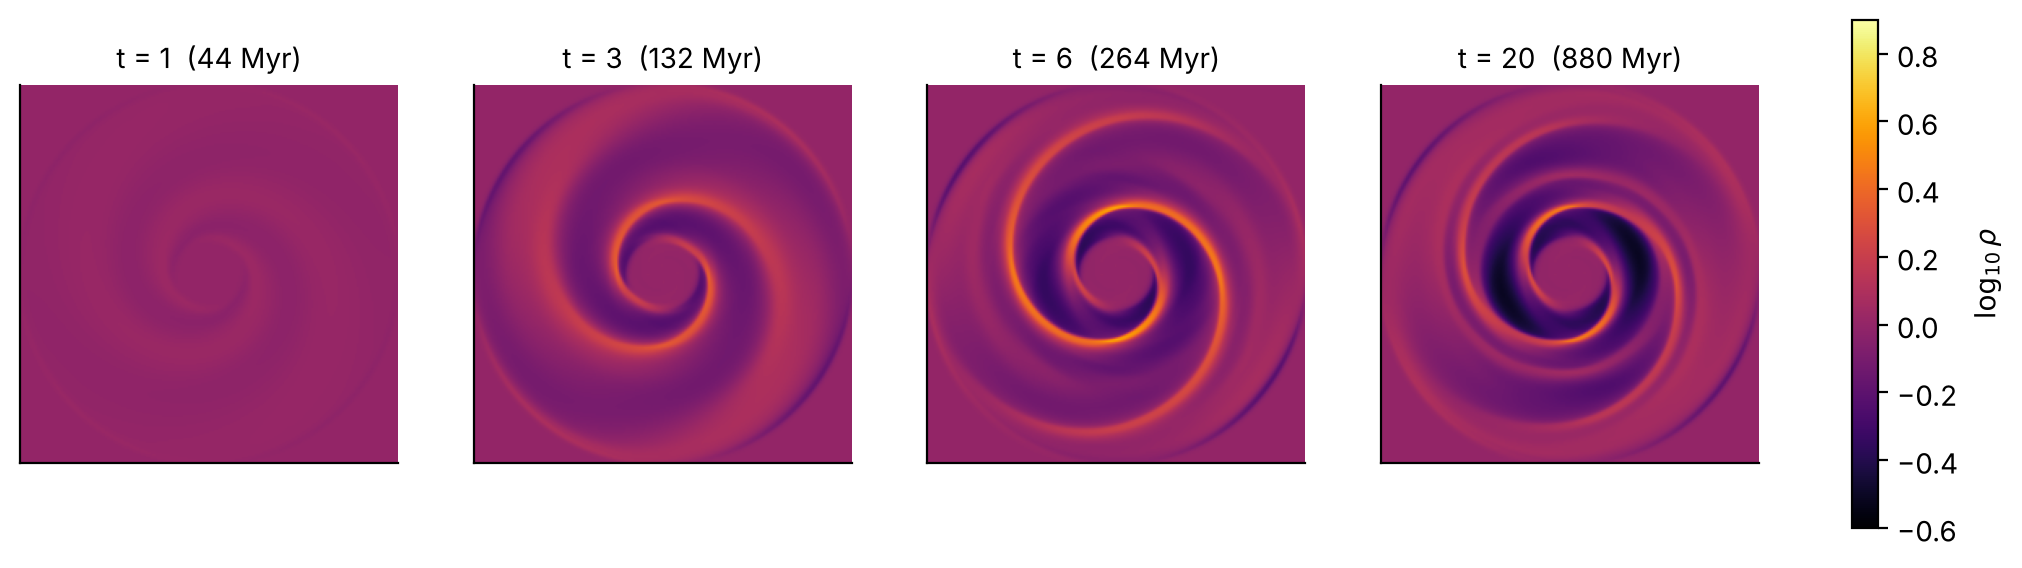
\includegraphics[width=\textwidth]{fig_snapshots.png}
\caption{Gas density ($\log_{10}\rho$) of the fiducial run at 44, 130, 260 and 880 Myr, in the frame rotating with the spiral pattern.}
\label{fig:snap}
\end{figure}

\subsection{The arms are shocks}
Around a ring at $r=0.45$ (Fig.~\ref{fig:profile}), the density rises steeply where gas enters an arm and decays slowly on the way out, giving a saw-tooth profile. At the same location, the velocity component normal to the arm, $u_\perp$, drops abruptly. A linear density wave would instead give a smooth, symmetric sinusoid.

The streamlines (Fig.~\ref{fig:stream}) bend sharply where they cross an arm. This is the behaviour of an oblique shock (A.14): the normal velocity component drops while the tangential component is continuous, so the flow is deflected.

\begin{figure}[H]
\centering
\begin{minipage}{0.56\textwidth}\centering
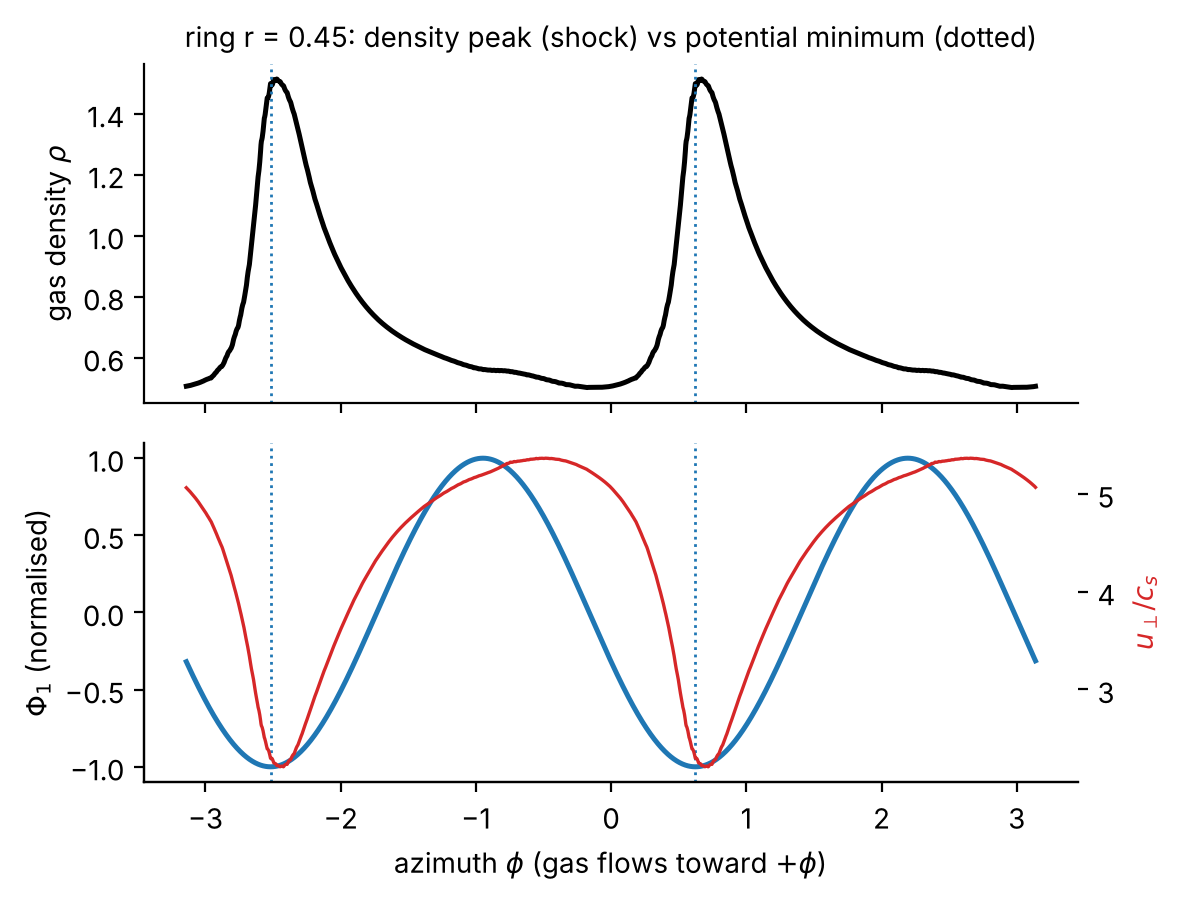
\includegraphics[width=\textwidth]{fig_profile.png}
\caption{Density, spiral potential and normal velocity around the ring $r=0.45$.}
\label{fig:profile}
\end{minipage}\hfill
\begin{minipage}{0.4\textwidth}\centering
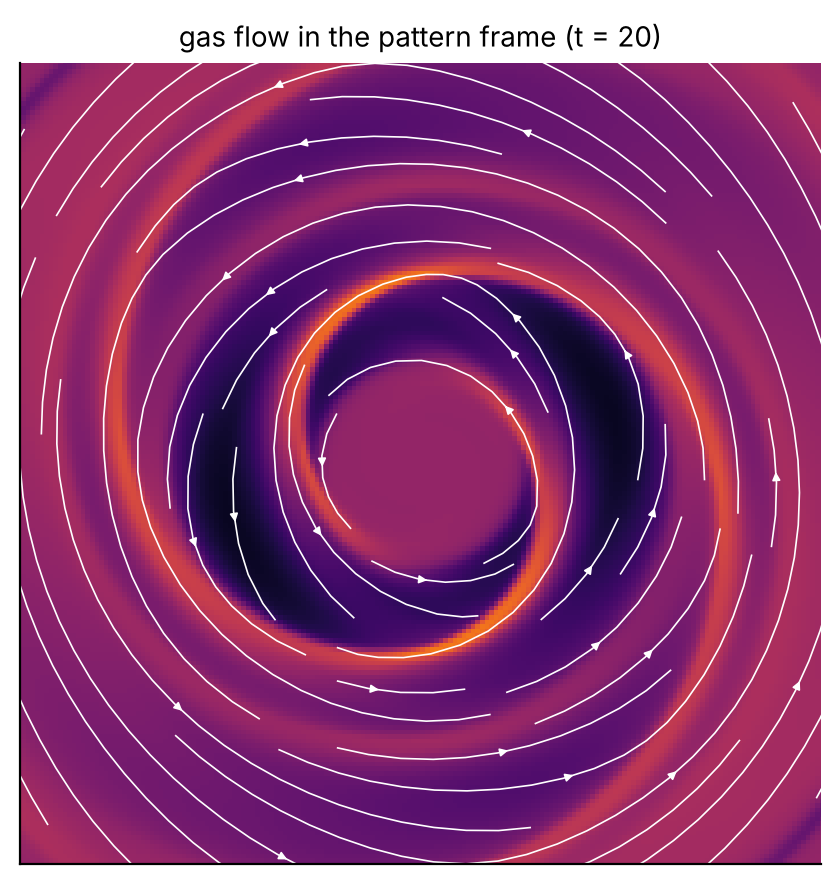
\includegraphics[width=\textwidth]{fig_streamlines.png}
\caption{Streamlines in the pattern frame bend sharply at the arms.}
\label{fig:stream}
\end{minipage}
\end{figure}

\subsection{Where the arms are strong}
In the pattern frame, gas reaches an arm with normal Mach number
\begin{equation}
\mathcal{M}_\perp\simeq\frac{(v_c-\Omega_p r)\sin i}{c_s}.
\end{equation}
This decreases outward, because the gas and the pattern rotate at more similar speeds, and it reaches $\approx1$ at $r\approx0.94$, just inside corotation. Figure~\ref{fig:radial} shows that the measured arm contrast follows $\mathcal{M}_\perp$ in the outer disk: the arms weaken as the inflow becomes only marginally supersonic. The strongest response is at $r\approx0.35$, next to the ILR, where the epicyclic motion of the gas resonates with the forcing.

\begin{figure}[H]
\centering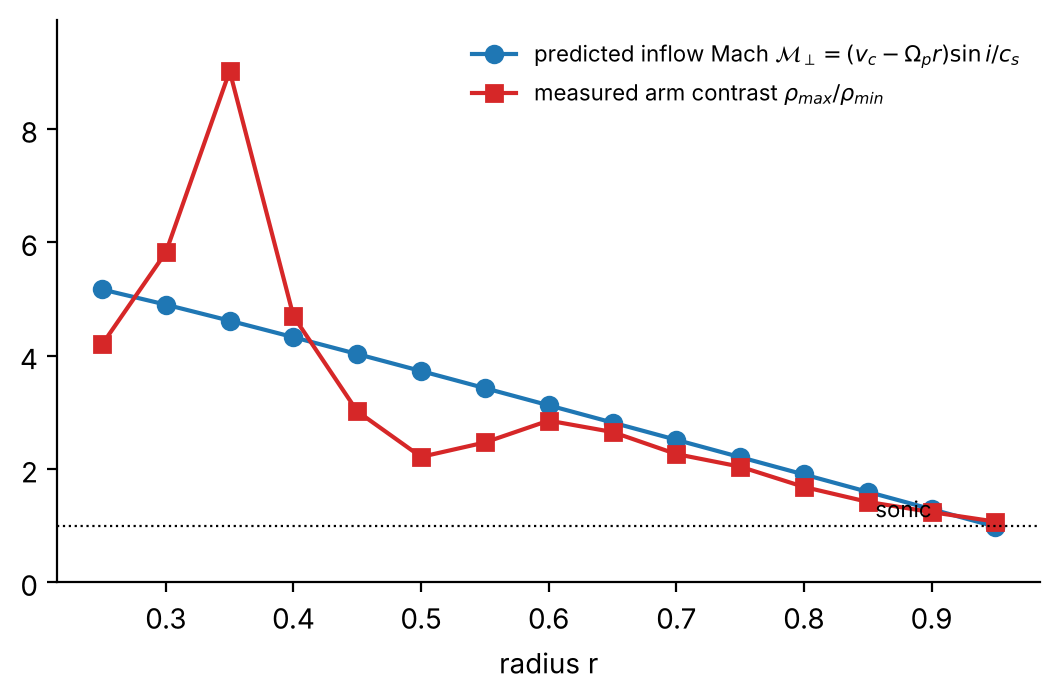
\includegraphics[width=0.62\textwidth]{fig_radial.png}
\caption{Predicted inflow Mach number $\mathcal{M}_\perp$ and measured arm contrast $\rho_{\max}/\rho_{\min}$ versus radius.}
\label{fig:radial}
\end{figure}

\subsection{What controls the arm strength}
\begin{itemize}[nosep]
\item \textbf{Weak forcing ($F\lesssim1\%$):} the response is a gentle wave whose contrast grows roughly $\propto F$, as expected from linear theory (Fig.~\ref{fig:forcing}).
\item \textbf{Stronger forcing:} the response grows faster than linearly and steepens into shocks.
\item \textbf{Gas temperature:} colder gas (lower $c_s$, higher $\mathcal{M}_\perp$) forms sharper and denser arms, while warm gas at $\approx22$ km\,s$^{-1}$ barely shocks (Fig.~\ref{fig:cs}). This is consistent with spiral arms being traced by cold, dense gas.
\end{itemize}

\begin{figure}[H]
\centering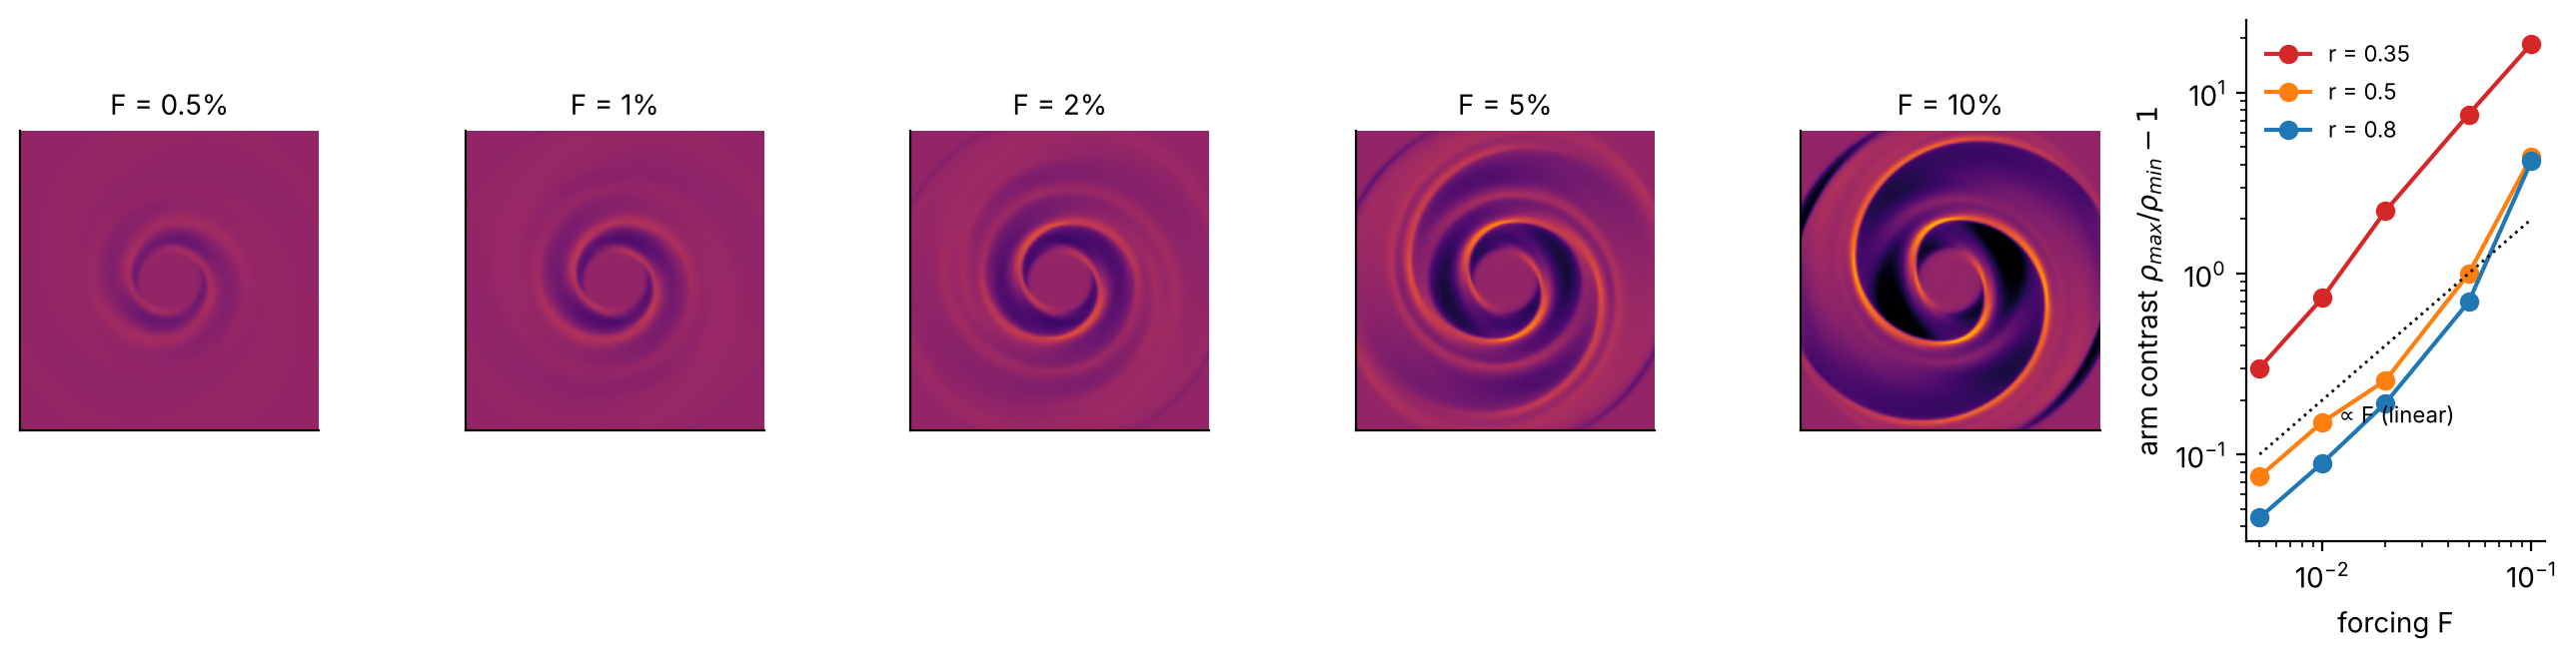
\includegraphics[width=\textwidth]{fig_forcing.png}
\caption{Gas density for spiral forcing $F=0.5$--$10\%$ (left five panels), and arm contrast versus forcing at three radii (right).}
\label{fig:forcing}
\end{figure}

\begin{figure}[H]
\centering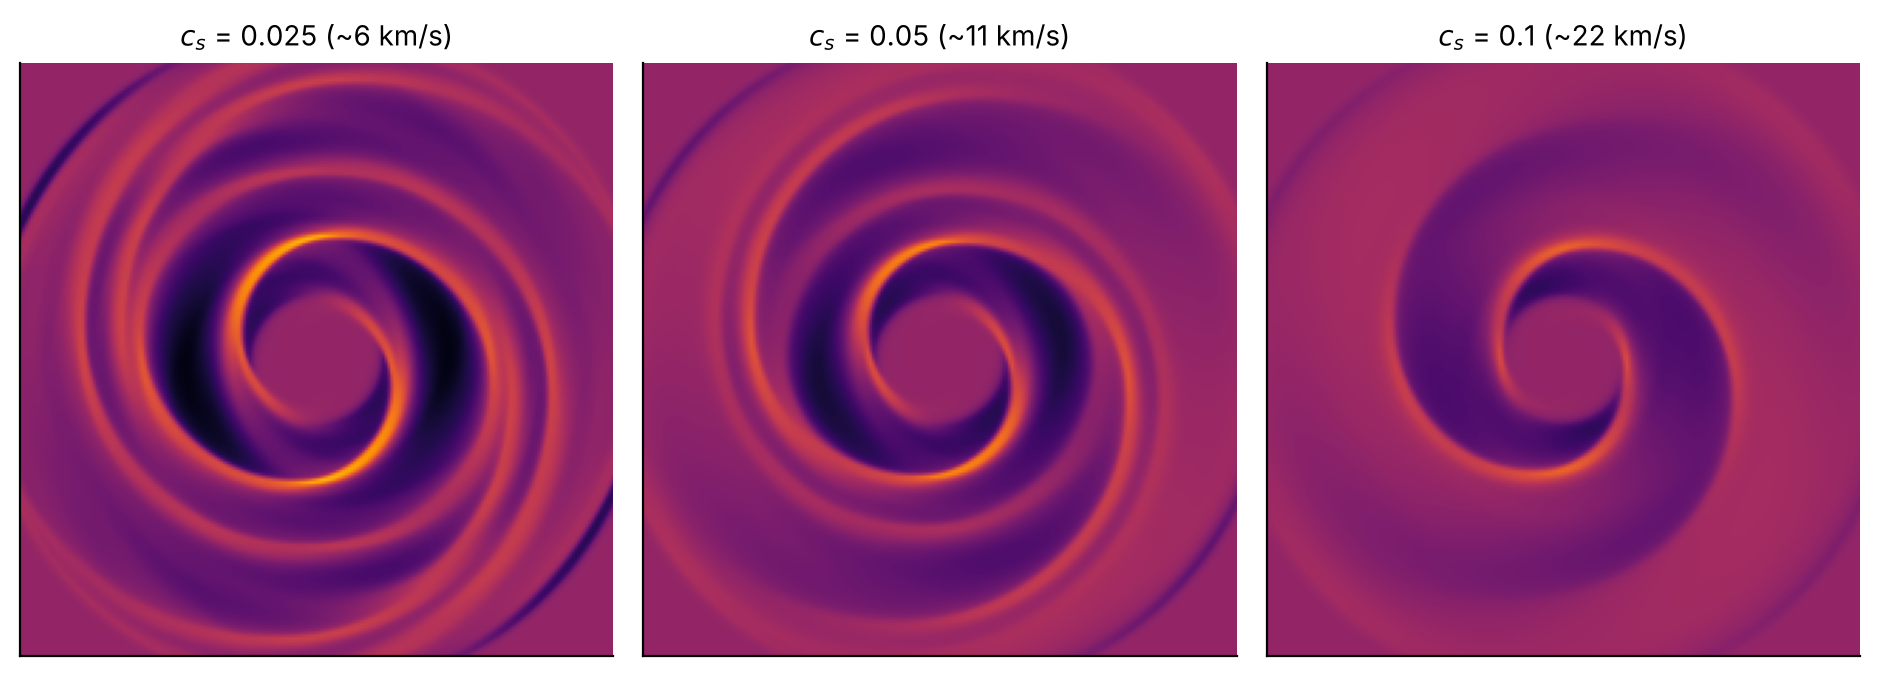
\includegraphics[width=0.8\textwidth]{fig_cs.png}
\caption{Gas density for sound speeds $c_s=0.025$, $0.05$ and $0.1$ (about 6, 11 and 22 km\,s$^{-1}$).}
\label{fig:cs}
\end{figure}

%=====================================================================
\section{Limitations}
\begin{itemize}[nosep]
\item \textbf{Resolution.} The arm \emph{positions} converge, but the peak density does not: it rises from 1.9 to 3.1 to 4.4 at $r=0.35$ for $N=128$, $256$, $512$ (Fig.~\ref{fig:res}). The shock is captured in a fixed number of cells, so it becomes thinner and denser on finer grids. This is the same numerical-diffusion effect seen in the HW2 Kelvin--Helmholtz growth rates.
\item \textbf{Physics.} The spiral is imposed, not self-consistent, and there is no self-gravity, cooling, magnetic field or star formation.
\item \textbf{Grid.} A fixed Cartesian grid is not Galilean invariant, so it adds diffusion where gas moves quickly across cells.
\end{itemize}

\begin{figure}[H]
\centering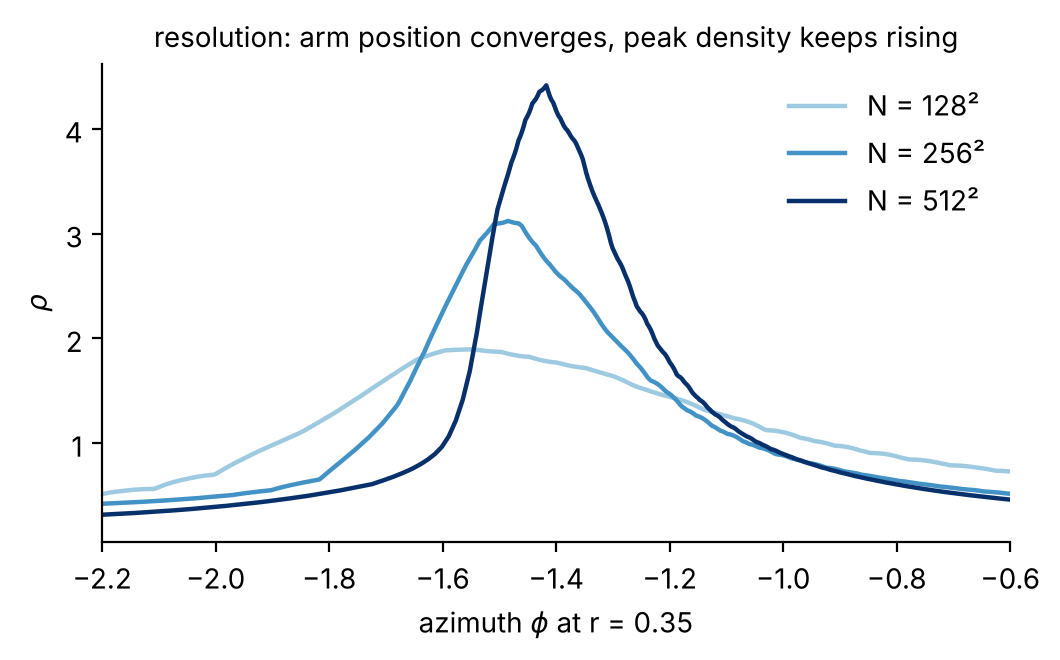
\includegraphics[width=0.55\textwidth]{fig_resolution.png}
\caption{Density around the ring $r=0.35$ for three resolutions.}
\label{fig:res}
\end{figure}

%=====================================================================
\section{Conclusions}
\begin{enumerate}[nosep]
\item The HW2 finite-volume solver, extended with gravity, rotating-frame forces and an isothermal equation of state, reproduces the classic result that \textbf{gas shocks at spiral arms}.
\item The solver reproduces the exact isothermal jump condition $D=\mathcal{M}^2$ to within 2\%.
\item The arm strength is set by the \textbf{inflow Mach number}: arms are strong in the inner disk and fade toward corotation. They are sharper for colder gas and stronger forcing.
\end{enumerate}
\textbf{Next steps:} add gas self-gravity (an FFT Poisson solver) so that arms can form spontaneously and the Toomre $Q$ criterion can be tested, and compare with a moving-mesh code.

{\sloppy\paragraph{Code.} The code and an executed notebook are in the project folder: the notebook \texttt{Spiral\_Arms.ipynb} shows all results, \texttt{spiral\_sim.py} contains the galaxy model, and \texttt{kh\_sim.py} is the HW2 solver it builds on.\par}

\begin{thebibliography}{9}
\bibitem[Lin \& Shu(1964)]{linshu64} Lin, C.~C., \& Shu, F.~H. 1964, \textit{ApJ}, 140, 646
\bibitem[Mocz(2020)]{mocz20} Mocz, P. 2020, \textit{Create Your Own Finite Volume Fluid Simulation (With Python)}, \url{https://github.com/pmocz/finitevolume-python}
\bibitem[Ogilvie(2016)]{ogilvie16} Ogilvie, G.~I. 2016, \textit{J. Plasma Phys.}, 82, 205820301 (arXiv:1604.03835)
\bibitem[Roberts(1969)]{roberts69} Roberts, W.~W. 1969, \textit{ApJ}, 158, 123
\end{thebibliography}

\end{document}
